\chapter{Historia}

\section{Antecedentes}

\noindent Las primeras formas fractales aparecieron en el siglo XIX, cuando el matemático Karl Weierstrass graficó en 1872 su famosa función de Weierstrass. Más tarde en ese mismo siglo, empezaron a surgir conceptos cada vez más cercanos a lo que hoy se consideran fractales, siendo más gemométricos y menos algebraicos.

\begin{figure}[H]
    \centering
    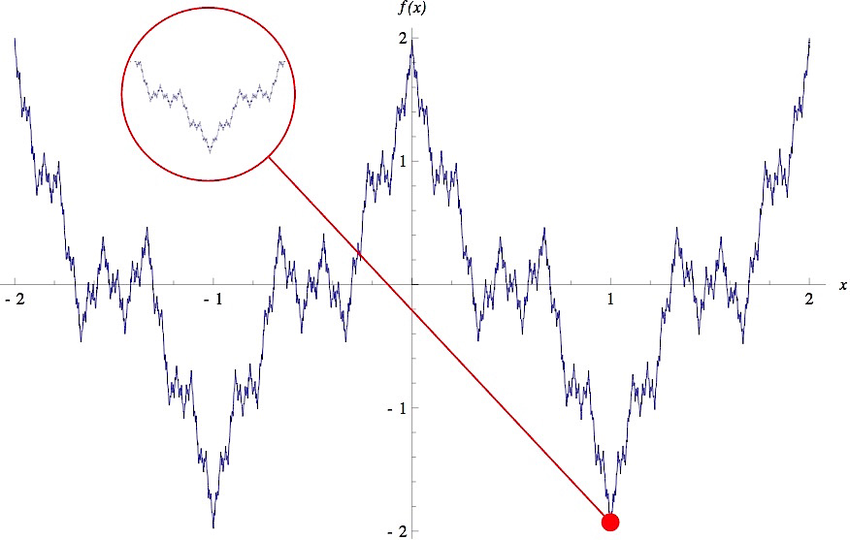
\includegraphics[width=0.5\textwidth]{figures/weierstrass-function.png}
    \caption{Función de Weierstrass}
    \label{fig:weierstrass-function}
\end{figure}

\section{Primeros fractales}

\noindent Así, en 1904, Helge von Koch definió su copo de nieve, una curva con propiedades similares a la de Weierstrass. En 1915, Waclaw Sierspinski construyó su triángulo y, un año después, su alfombra.

\begin{figure}[H]
    \centering
    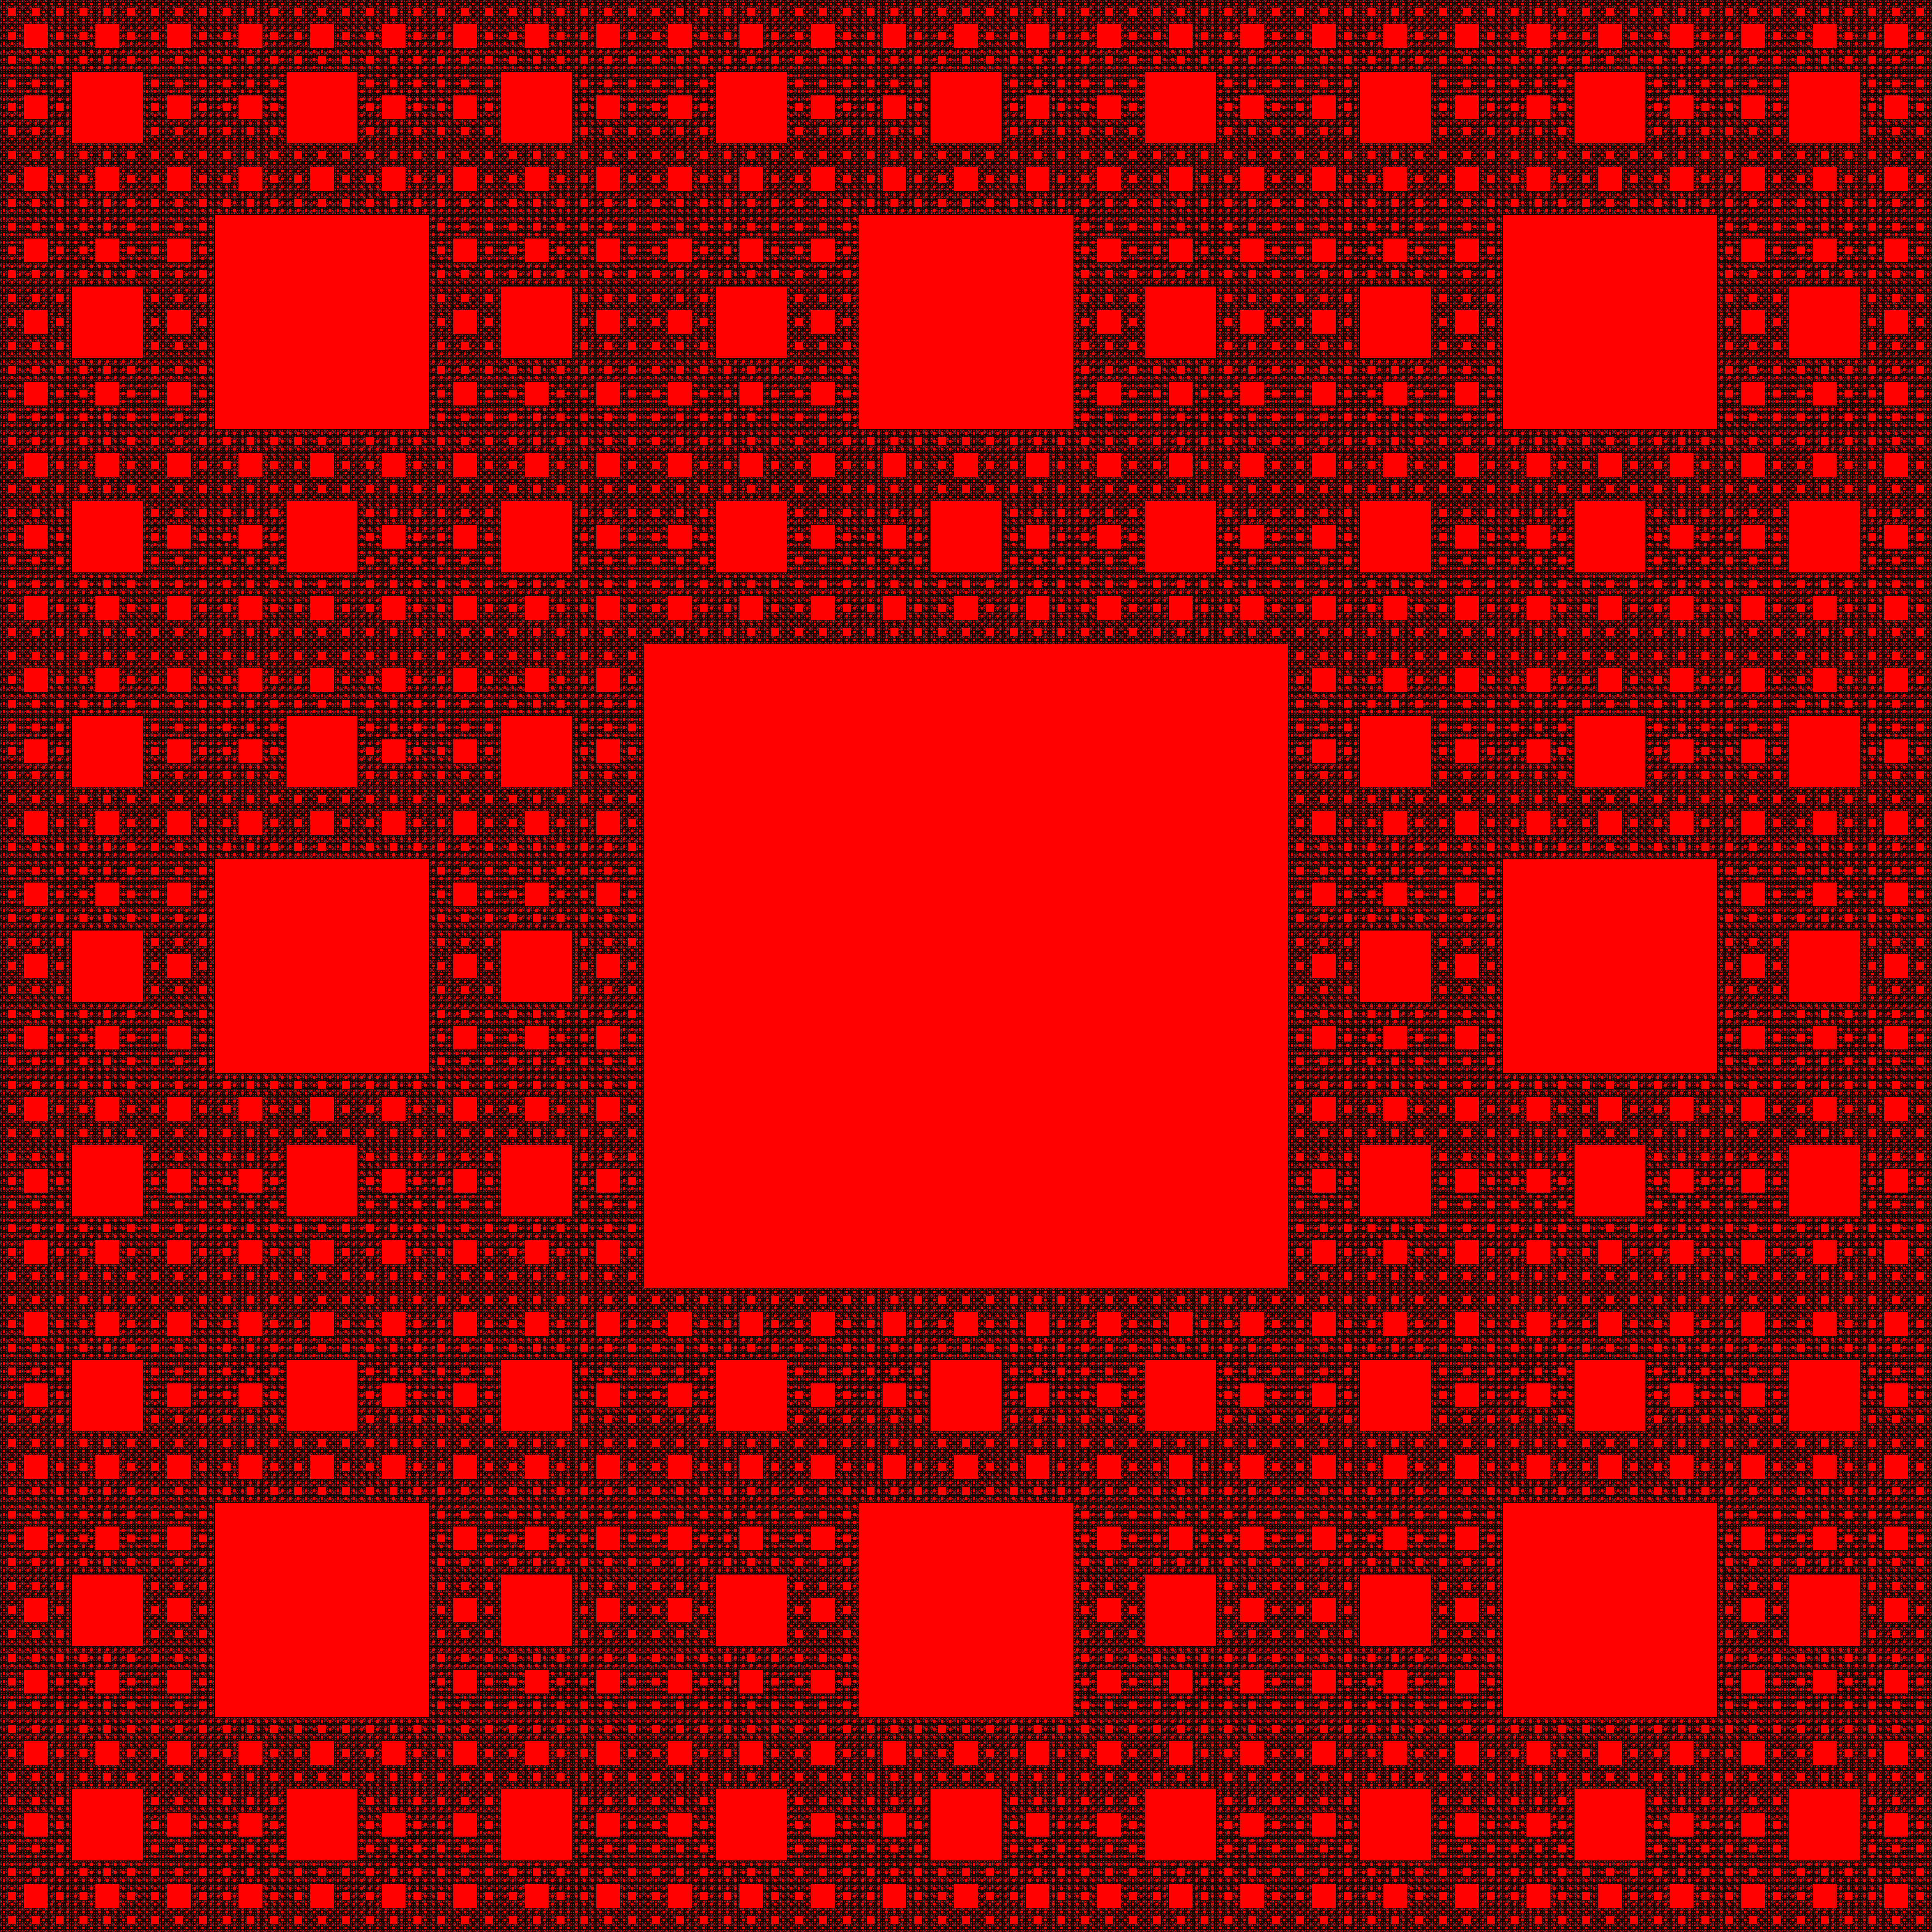
\includegraphics[width=0.5\textwidth]{figures/sierspinsky-carpet.png}
    \caption{Alfombra de Sierspinsky}
    \label{fig:sierspinsky-carpet}
\end{figure}

\section{Nuevas matemáticas}

\noindent En el siglo XIX, Georg Cantor desarrolló su conjunto de Cantor y 
Giuseppe Peano su curva de Peano.Gracias a esto se dieron cuenta de que estos objetos matemáticos no eran casos particulares, si no que había un gran conjunto de funciones que compartían las mismas cualidades que la función de Weierstrass.\\

\begin{figure}[H]
    \centering
    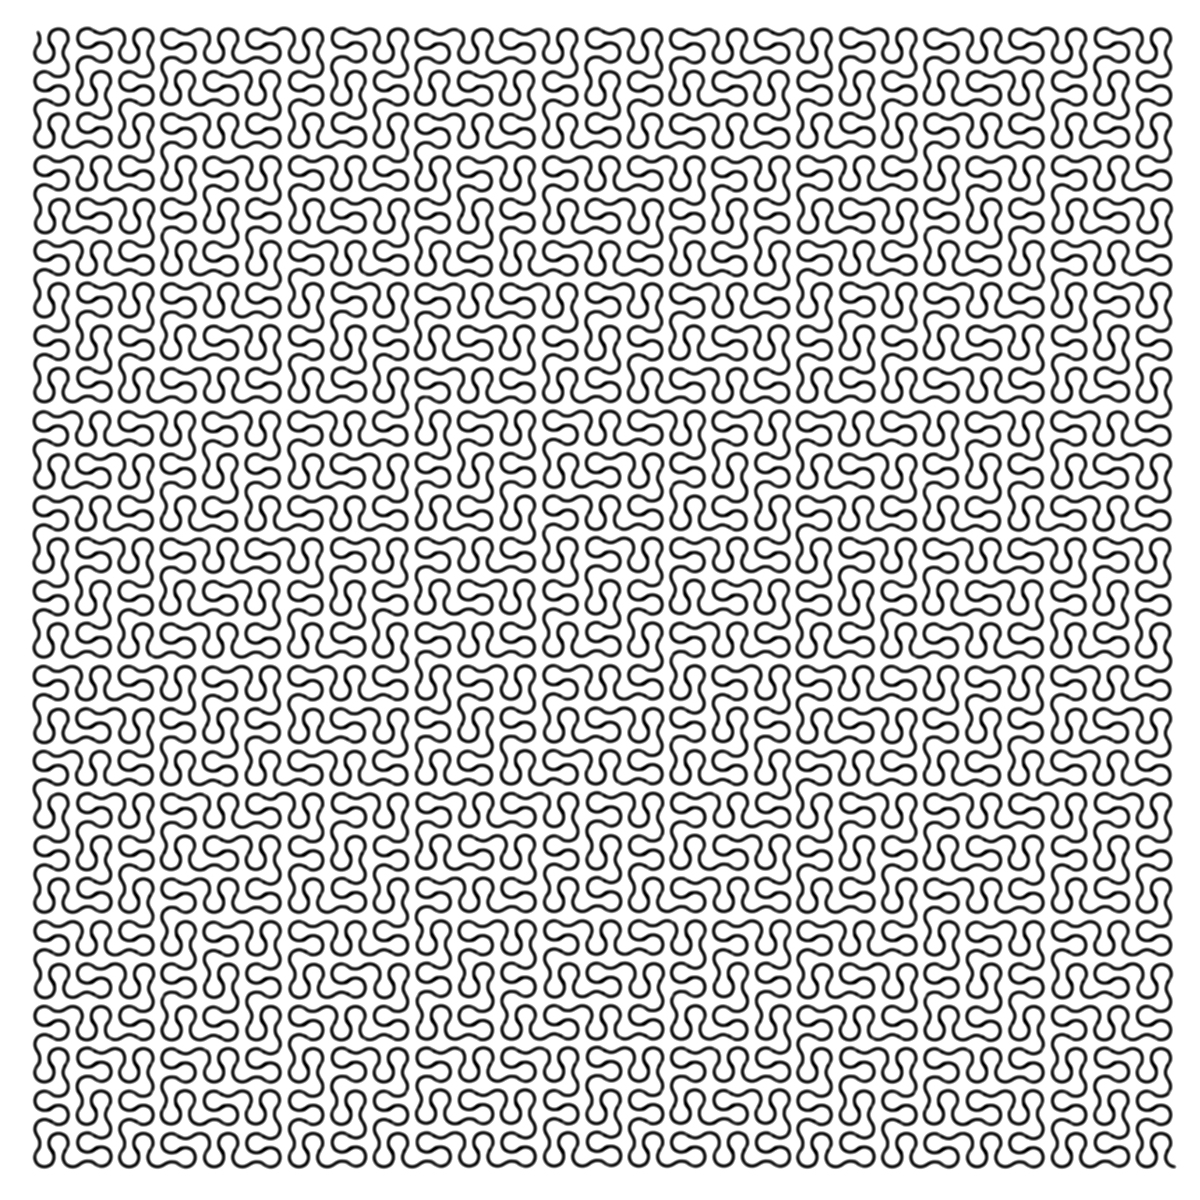
\includegraphics[width=0.5\textwidth]{figures/peano-curve.jpg}
    \caption{Curva de Peano}
    \label{fig:peano-curve}
\end{figure}


\noindent A pesar de que hubiese un gran conjunto de funciones, la geometría de Euclides y la dinámica Newtoniana no podían describirlas bien. En 1919, el matemático Félix Hausdorff introdujo la primera manera de observar y estudiar estos objetos, la dimensión de Hausdorff-Besicovitch. Años más tarde, Andrei Kolmogorov describió una herramienta similar conocida como la entropía de Kolmogorov.

\noindent En 1963, Benoît Mandelbrot empezo a trabajar con los fractales a raíz de otra investigación, lo que le llevó a fundar la geometría fractal.

\section{Mandelbrot}

\noindent Mandelbrot es uno de los mayores exponentes en el avance del campo de los fractales, desde identificar una muestra de \textit{"tiempo fractal"} hasta replantearse un problema mundialmente conocido: ¿Cuál es la longitud de la costa de Gran Bretaña? Según Mandelbrot esta distancia es infinita, o mejor dicho, depende de la longitud de la regla con la que se mida. Como ya hemos comentado, la geometría euclídea no es capaz de describir estos objetos, por lo que Mandelbrot utilizó la noción de dimensión, y en concreto, la extraña definición de dimensión fraccionarias.\\

\noindent En 1975, Mandelbrot acuñó el término fractal, que proviene del latín \textit{fractus}, que significa roto o fracturado. El fractal más famoso de Mandelbrot es el conjunto de Mandelbrot, el cual es el más estudiado dentro del campo.

\begin{figure}[H]
    \centering
    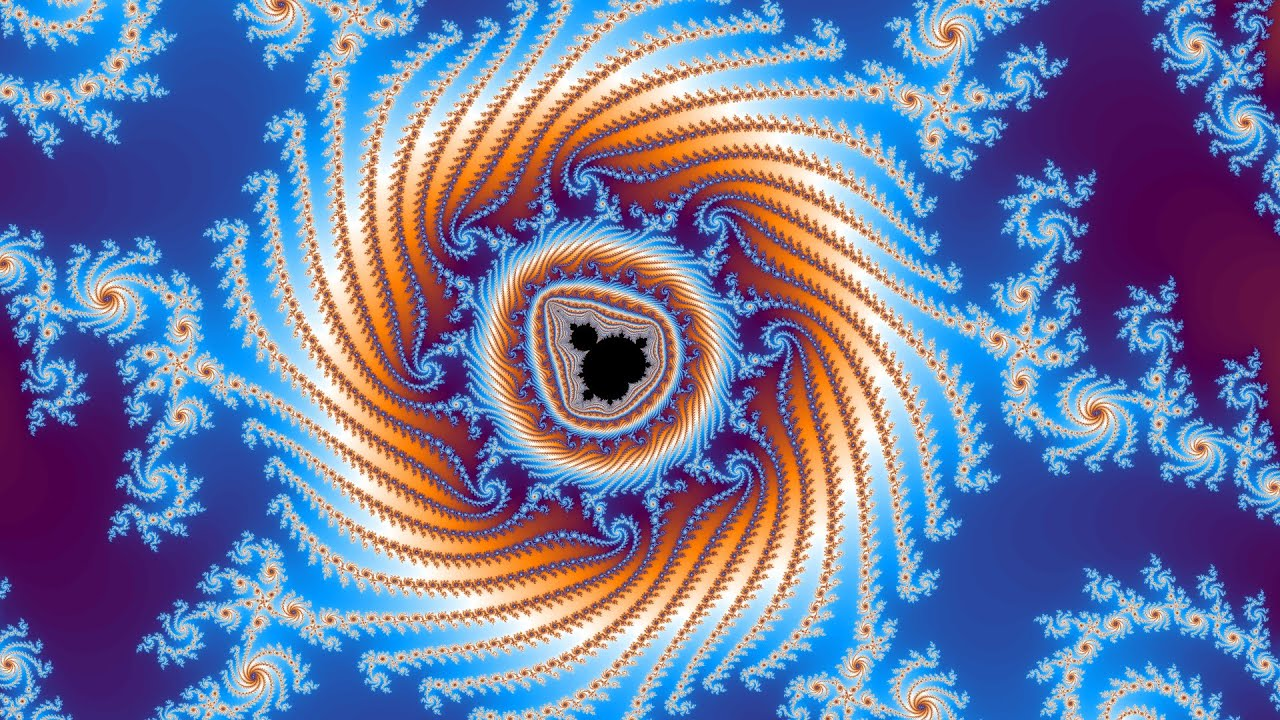
\includegraphics[width=0.5\textwidth]{figures/mandelbrot-set-1.jpg}
    \caption{Conjunto de Mandelbrot}
    \label{fig:mandelbrot-set}
    
\end{figure}